%!TEX root = ../main.tex

\section{Studies of systematic effects}
\label{sec:b02dd:systematics}

%============================================================================%
\subsection{Cross-checks}
\label{sec:b02dd:systematics:xchecks}
To check for possible systematic effects, fits in different subsamples of the
nominal data set are performed. The cross-checks are performed for the two
tagging algorithms (OS vs. SS (not exclusive samples)), the two years of
data-taking (2011 vs. 2012) , combinations of those, the magnet polarities (Up
vs. Down), the two final states ($\KpipiKpipi$ vs. $\KKpiKpipi$) and for four
different slices of the BDT classifier for the $\KpipiKpipi$ final state.

\begin{figure}[thb]
\centering
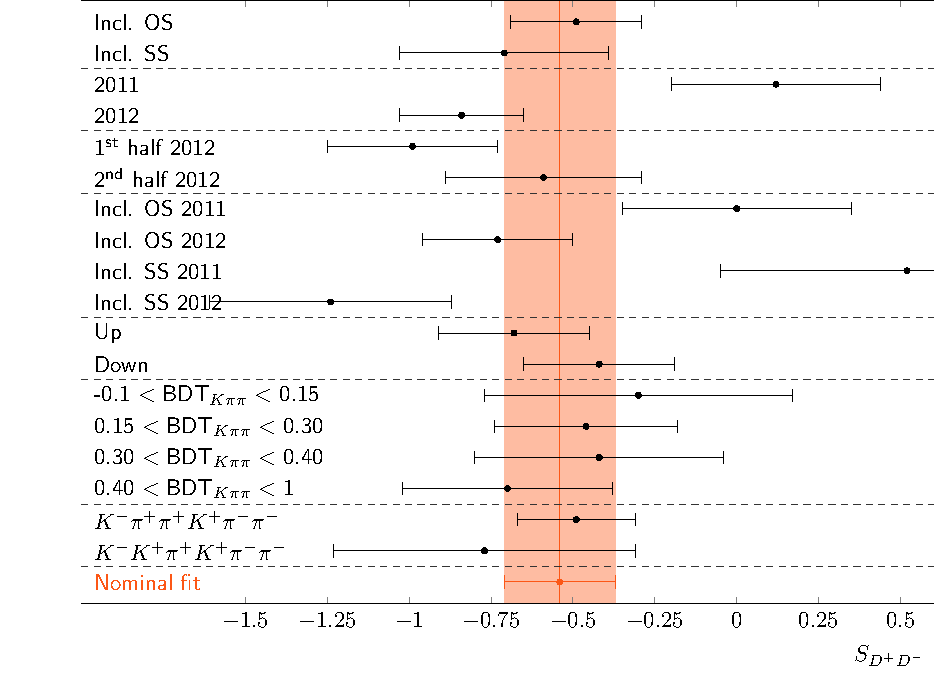
\includegraphics[width=0.9\textwidth]{07-B02DD/tikz/pdf/SComparison.pdf}
\caption{
Comparison of fit results of \SDD for fits on various subsamples.}
\label{fig:b02dd:systematics:xchecks:subsamples:s}
\end{figure}
\begin{figure}[thb]
\centering
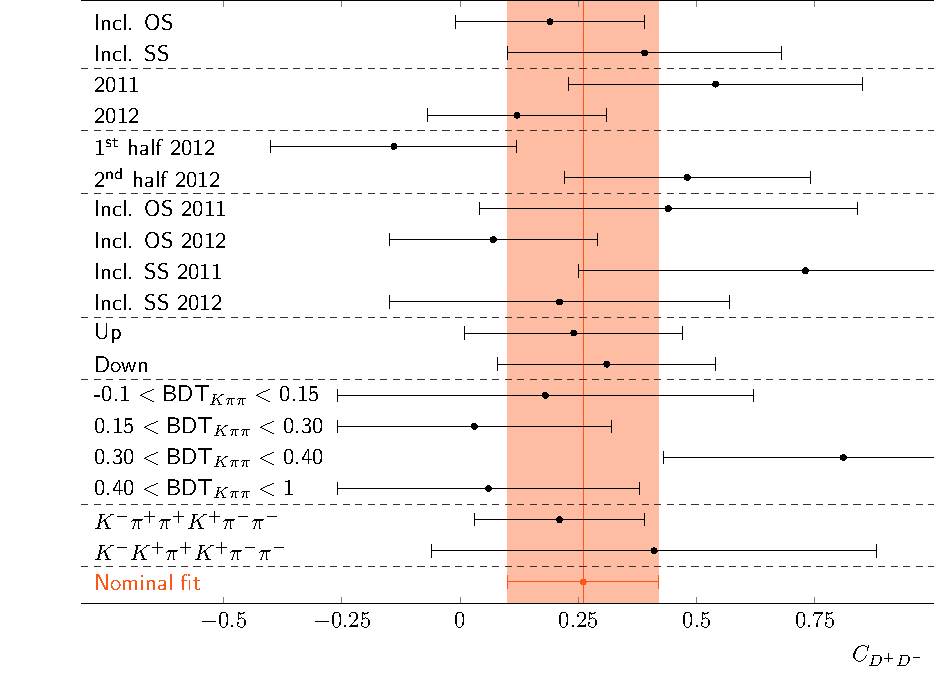
\includegraphics[width=0.9\textwidth]{07-B02DD/tikz/pdf/CComparison.pdf}
\caption{
Comparison of fit results of \CDD for fits on various subsamples.}
\label{fig:b02dd:systematics:xchecks:subsamples:c}
\end{figure}
The fit results in the various scenarios are illustrated in
\cref{fig:b02dd:systematics:xchecks:subsamples:s,fig:b02dd:systematics:xchecks:subsamples:c}.
While almost all splits show compatible results, a rather large difference can
be observed between the 2011 and the 2012 subsample for $\SDD$. This is even
more pronounced when using only SS tagging. However, when calculating the
difference of the log likelihoods it turns out that the two results are
compatible within \num{2.6} standard deviations. Nevertheless, the
flavour-tagging calibration parameters are also determined separately for 2011
and 2012 data. Only small non-significant differences are observed, which can
not explain the different results of the $\CP$ observables. Therefore, the
best explanation is that the difference is due to a statistical fluctuation.

For the nominal fit the decay times and the decay time errors from the
DecayTreeFitter (DTF) are used. The central values of the $\CP$ observables
slightly change when using the decay time (error) from the LoKiVertexFitter
(LVF), $\SDD = \num{-0.539}$ (LVF) vs. \num{-0.541} (DTF) and $\CDD =
\num{0.266}$ (LVF) vs. \num{0.263} (DTF). But this difference is clearly below
the statistical significance.

\FloatBarrier

%============================================================================%
\subsection{Decay time fit bias}
\label{sec:b02dd:systematics:fitbias}

The likelihood fit itself might be biased. The nominal fit results for the
$\CP$ observables are used to generate \num{10000} pseudoexperiments. The pull
distributions in \cref{fig:b02dd:systematics:fitbias:pulls} show a very small
deviation of the mean value from zero.
%
\begin{figure}[htb]
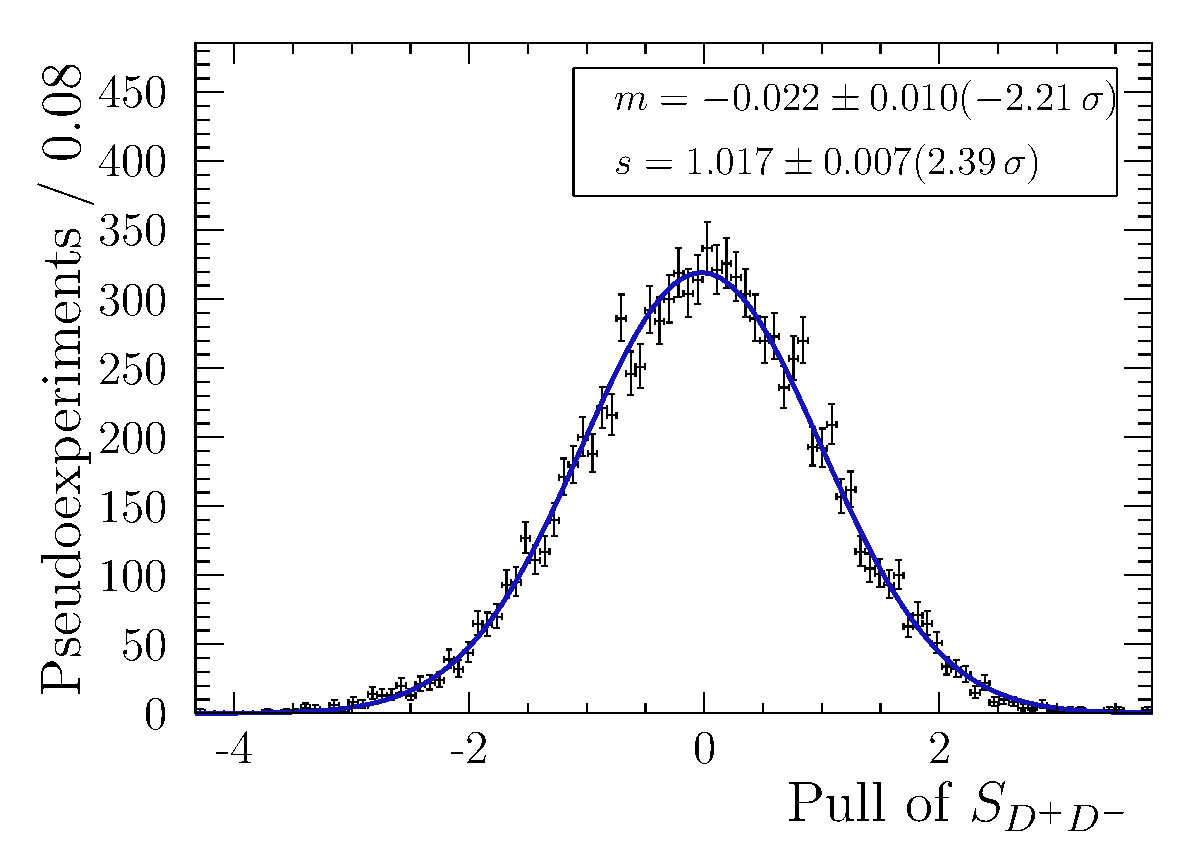
\includegraphics[width=0.49\textwidth]{07-B02DD/tikz/pdf/parSigTimeSin2b_pull_fitbias.pdf}
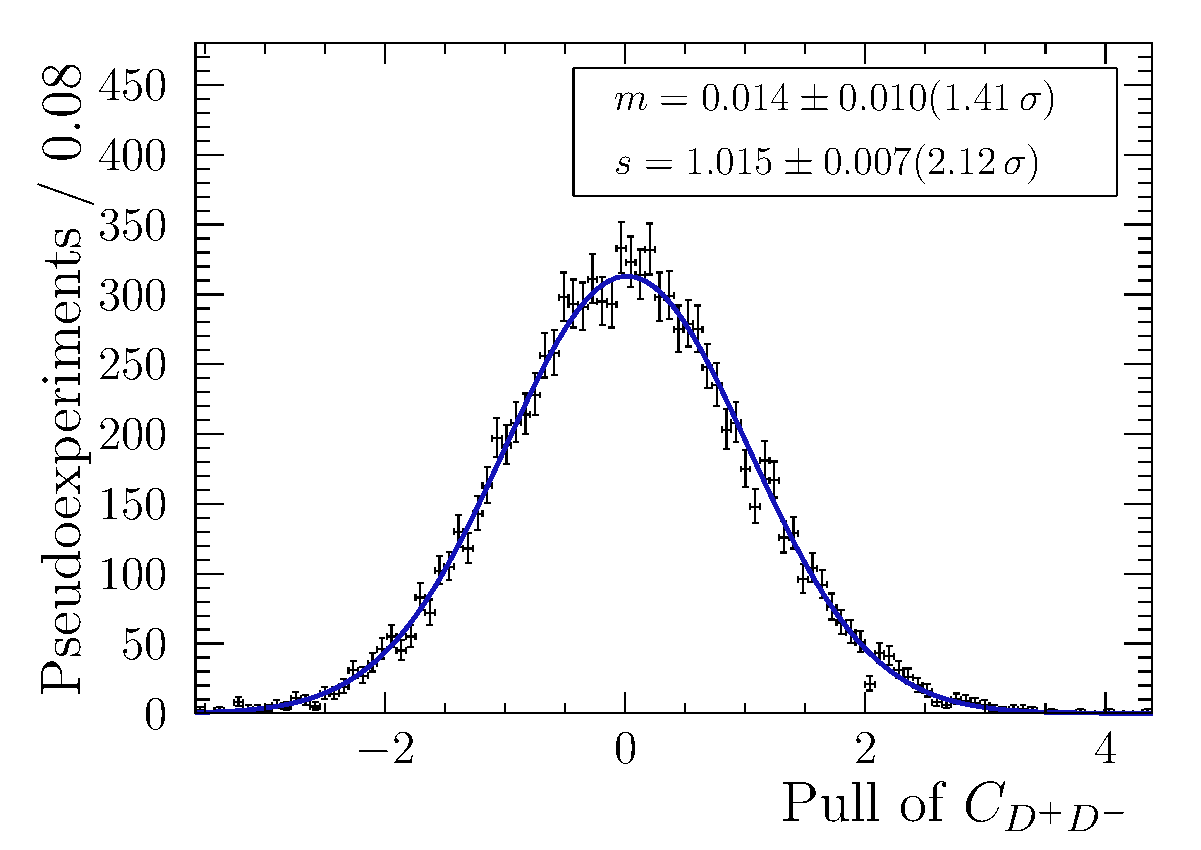
\includegraphics[width=0.49\textwidth]{07-B02DD/tikz/pdf/parSigTimeC_pull_fitbias.pdf}
\caption{Pull distributions of $\SDD$ and $\CDD$ for a study on the systematic
uncertainty due to the likelihood fitter.}
\label{fig:b02dd:systematics:fitbias:pulls}
\end{figure}
%
Multiplying it with the statistical uncertainty the systematic uncertainty is
calculated to be
\begin{align}
s_{\SDD}^{\textrm{fit}} = \num{0.004}\ , \qquad s_{\CDD}^{\textrm{fit}} = \num{0.0025}\ .
\end{align}
For all following studies of systematic uncertainties the residuals are
corrected for the decay time fit bias. Otherwise, even effects that are
actually not biasing would be misinterpreted due to the fit bias.

%============================================================================%
\subsection{Fit model}
\label{sec:b02dd:systematics:fitmodel}
%!TEX root = ../main.tex

%----------------------------------------------------------------------------%
\subsubsection{Mass Model}
\label{sec:b02dd:systematics:massmodel}

Two different aspects of the mass model are studied regarding systematic
uncertainties: the impact of neglecting contributions and of mismodelling
components.

\paragraph{Neglected contributions}

If a neutral \piz or a photon is missed in the reconstruction the decay
\BToDstD, with \DstpToDpizero or \DstpToDgamma, can mimic the \BToDD decay. In
the rest frame of the \Dstarp resonance, the missing momentum of the \piz is
fixed, but it needs to be boosted when transferred into the rest frame of the
\PB meson. So, the reconstructed mass depends on the helicity angle of the
missing \piz. This leads to a double-horned structure approximately
\SI{140}{\MeVcc} below the nominal \PB mass (see Ref.~\cite{LHCb-ANA-2014-015}
for more details on the shape of this background). As the lower boundary on
the invariant $m_{\Dp\Dm}$ mass is set to \SI{5150}{\MeVcc} the \BdToDstD
contribution lies outside the mass range used for the fit. However, the
\BsToDstD contribution enters the fit region. But since the expected number of
\BsToDstD candidates is low, it is not included in the nominal mass model.
Another contribution that is neglected in the nominal mass fit model is
(partially) charmless background where at least one of the hadron triplets is
not originating from a \PD decay. The systematic uncertainty on the
determination of the \CP observables arising from neglecting these two
contributions is estimated using \num{1000} pseudoexperiments. Components for
\BsToDstD and for (partially) charmless background are included in the
generation but excluded from the fit procedure.

The shape of \BsToDstD is parametrised with two single Gaussian functions
centred around \SI{5150}{\MeVcc} and \SI{5200}{\MeVcc}. The (partially)
charmless background is modelled with a single Gaussian function. When
optimising the decay time significance cut it has been observed that the width
of the (partially) charmless background is approximately \SI{10}{\percent}
wider than the signal component. Therefore, a width of \SI{10}{\MeVcc} is
chosen. The mean is set to the same position as the \Bd signal. The \BsToDstD
component is generated without any tagging asymmetry, while for the (partially)
charmless background the worst case scenario of maximal \CP violation with the
opposite \CP eigenvalue ($S_f = \num{+1.0}$) is tested.

In studies of \BdToDstD decays~\cite{BToDstDthesis} a significant contribution
of \BsToDstD candidates is observed. The ratio between the two yields is
determined to be 1:20. Under the assumption that the efficiencies for \BToDD
and \BToDstD are the same the expected number of \BsToDstD candidates can be
calculated via
\begin{align}
	\text{N}_{\BsToDstD} = \frac{1}{20} \text{N}_{\BdToDD} \frac{\mathcal{B}(\BdToDstD) \mathcal{B}(\Dstarp \!\to \Dp (\piz || \gamma))}{\mathcal{B}(\BdToDD)} \,.
\end{align}
Using the world averages for the branching ratios~\cite{PDG2016} the number of
candidates to be generated in the pseudoexperiments is estimated to be
N(\BsToDstD) = \num{66\pm9}.

To determine how many (partially) charmless background candidates need to be
generated the $D$ mass window is widened to $\SI{\pm40}{\MeVcc}$ and the
nominal $D$ mass window of $\SI{\pm25}{\MeVcc}$ is vetoed for one or for both
$D$ candidates. Fits to the invariant $B$ mass without the $D$ mass constraint
are performed in the various scenarios. % yielding
% $\num{0.0\pm2.6}\,\mbox{\Bd\!\to\KpipiKpipi}$ candidates,
% $\num{0.0\pm9.2}\,\mbox{\Bd\!\to\KKpiKpipi}$ candidates,
% $\num{0.0\pm4.9}\,\mbox{\Bd\!\to\D(\Kpipi)\Kpipi}$ candidates,
% $\num{0.0\pm3.3}\,\mbox{\Bd\!\to\D(\KKpi)\Kpipi}$ candidates, and
% $\num{17.2\pm11.2}\,\mbox{\Bd\!\to\D(\Kpipi)\KKpi}$ candidates.
%
The fitted yields, which are constrained to positive values, are scaled to
account for the applied $D$ mass window. The total amount of residual
contamination ($\Bz\!\to\PD hhh$ or $\Bz\!\to hhhhhh$ decays) surviving the
\BdToDD selection is found to be $\num{28.7\pm19.5}$ candidates for the
$\KKpiKpipi$ final state and $\num{0.0\pm27.8}$ candidates for the
$\KpipiKpipi$ final state. For the pseudoexperiments the number of (partially)
charmless background is drawn from Gaussian distributions using these values
for mean and width. When the outcome is negative the procedure is repeated,
until a positive yield is drawn.

The systematic uncertainties on \SDD and \CDD are calculated as the product of
the bias on the mean parameter of the pull distributions and the statistical
uncertainty:
\begin{align*}
s_{\SDD}^{\text{mass,1}} = \num{0.05}\ , \qquad s_{\CDD}^{\text{mass,1}} = \num{0.013}\,.
\end{align*}

\paragraph{Mismodelling of mass components}

The BDT is trained with MC samples that are known to not perfectly model the
PID information. As a result the BDT classifier distributions of
background-subtracted data and MC show a quite big discrepancy. Some shape
parameters are estimated on MC samples and might be distorted by the data/MC
differences. Therefore, different alternative mass parametrisations are tested
against the nominal model: the component of the \BdToDD signal (and of the
\BsToDD background) is parametrised with a single Gaussian function; the
combinatorial background is described with a second order Chebyshev polynomial
of first kind; the tail parameters of \BToDsD are once extracted from the MC
sample without applying the BDT and once applying a tight cut on the BDT
classifier. The mass fit is performed with these new models, sWeights are
calculated for each approach, and the decay time fit is performed. The results
of the \CP observables are then compared with the nominal central values. The
largest deviations for \SDD and \CDD are
\begin{align*}
s_{\SDD}^{\text{mass,2}} = \num{0.004}\ , \qquad s_{\CDD}^{\text{mass,2}} = \num{0.006}\,.
\end{align*}

%----------------------------------------------------------------------------%
\subsubsection{Correlation between decay time and mistags}
\label{sec:b02dd:systematics:correlation_mistag_time}

The correlation between the decay time distribution and the per-event mistags
is studied by calculating the linear Pearson correlation coefficient
$\rho(\eta,t)$. The significance of the correlation value, \ie
\SI{95}{\percent} confidence level interval, is determined using the
bootstrapping method (\cref{sec:dataanalysis:bootstrapping}) with \num{10000}
repetitions. The correlation coefficients are found to be small. The profile
histogram of the OS tagging combination, which shows the average \etaos value
as a function of the decay time, is flat within statistics. For the SS tagging
combination the profile histogram slowly increases with decay time. This can
be confirmed by analysing the larger signal MC sample (see
\cref{fig:b02dd:systematics:correlation_mistag_time:etass_time_profile_MC}).
\begin{figure}[htb]
\centering
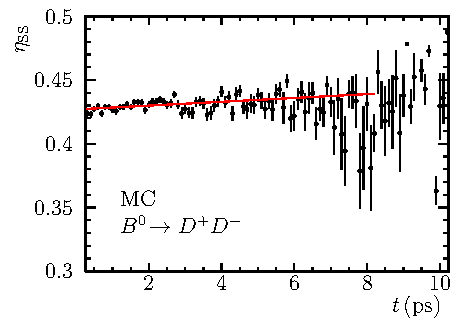
\includegraphics[width=0.6\textwidth]{07-B02DD/tikz/pdf/Profile_DecayTime_SS.pdf}
\caption{Profile histogram for the decay time dependence on $\etass$ for
signal MC. The black data points represent the mean value of $\etass$ and its
uncertainty for each bin in $t$. The red curve is the fitted linear function.}
\label{fig:b02dd:systematics:correlation_mistag_time:etass_time_profile_MC}
\end{figure}
Performing a $\chisq$ fit in the decay time range \SIrange{0.25}{8.25}{\ps}
with the linear function
\begin{align}
  \etass = a_{\etass,t} t + b_{\etass,t}
  \label{eq:tagging:correlation_mistag_time}
\end{align}
yields a slope of $a_{\etass,t} = \SI{1.50\pm0.27}{\invns}$. Although this is
a significant deviation from zero, the correlation is not taken into account in
the nominal fit model. Instead, a study on the systematic uncertainty from
neglecting this effect is performed. In \num{1000} pseudoexperiments the SS
mistag is generated using a Gaussian distribution whose mean is drawn from the
linear function defined in \cref{eq:tagging:correlation_mistag_time} thereby
introducing the correlation with the decay time. In the subsequent fit the
correlation is again ignored. This leads to systematic uncertainties of
\begin{align*}
s_{\SDD}^{\text{corr}} = \num{0.0007}\ , \qquad s_{\CDD}^{\text{corr}} = \num{0.007}\,.
\end{align*}

%----------------------------------------------------------------------------%
\subsubsection{Decay Time Resolution Model}
\label{sec:systematics:decaytimeresolution}

As calculated in \cref{sec:b02dd:decaytimefit:resolution} even an
underestimation of the decay time resolution by \SI{15}{\percent} has only a
minor effect on the resolution related dilution. Nevertheless, \num{1000}
pseudoexperiments are performed, in which the scale factors and the offset
parameters ($b_i$ and $c_i$ from \cref{tab:b02dd:decaytimefit:resolution}) are
enlarged by \SI{15}{\percent} in the generation and fixed to their nominal
values in the fit. Additionally, the mean parameter of the Gaussians is set to
the value obtained in the MC study for the generation and, like in the nominal
setup, fixed to zero in the fit. The systematic uncertainties are calculated
as the product of the biases on the mean parameter and the statistical
uncertainty to be
\begin{align*}
s_{\SDD}^{\text{res}} = \num{0.0020}\ , \qquad s_{\CDD}^{\text{res}} = \num{0.0023}\,.
\end{align*}

%----------------------------------------------------------------------------%
\subsubsection{Decay Time Acceptance Model}
\label{sec:systematics:decaytimeacceptance}

On signal MC the decay time acceptance is determined separately for the two
final states (see \cref{fig:b02dd:decaytimefit:acceptance_MC}). Small
differences are observed. As the low statistics in the \KKpiKpipi final state
on data does not allow for an individual spline model, a study is performed to
estimate a possible systematic uncertainty from neglecting this difference. In
\num{1000} pseudoexperiments the decay time distribution is generated using
the histograms of the true decay time acceptance from signal MC, split by
final state, and fitted with the spline acceptance as done in the nominal fit.
The use of the histograms with \num{100} bins should also cover uncertainties
from the choice of the number and position of the knots. The pull between the
fit results and the generation values is calculated. The systematic
uncertainty due to the decay time acceptance model is calculated as the
product of the shift in the pull distribution and the statistical uncertainty
of the nominal fit:
\begin{align*}
s_{\SDD}^{\textrm{acc}} = \num{0.007}\ , \qquad s_{\CDD}^{\textrm{acc}} = \num{0.0027}\,.
\end{align*}


%============================================================================%
\subsection{Further studies}
\label{sec:b02dd:systematics:others}
%!TEX root = ../main.tex

%----------------------------------------------------------------------------%
\subsubsection[\texorpdfstring{$z$}{z}-scale]{\texorpdfstring{$\boldsymbol{z}$}{z}-scale}
\label{sec:b02dd:systematics:z_scale}

The decay times are determined by measuring the distance between PV and decay
vertex. So, any uncertainty on the positioning of detector elements
(especially the VELO modules) leads to biased decay times. Due to the high
boosting the main contribution to the flight distance is in $z$ direction. The
scale uncertainty in $z$ direction has been estimated to be
$\sigma_{z\text{-scale}} = \SI{0.022}{\percent}$~\cite{LHCb-ANA-2011-055}. The
influence on the measurement of the \CP observables is studied by performing
\num{1000} pseudoexperiments. For each pseudoexperiment a value for the uncertainty
on the $z$-scale is drawn from a Gaussian distribution around zero of width
$\sigma_{z\text{-scale}}$. The sum of \SI{50}{\fs} and the product of this
value with the decay time is used as width of the Gaussian function modelling
the decay time resolution in the generation. In the fit the width is set to
\SI{50}{\fs}. The product of the bias from the pull distributions of the
pseudoexperiments and the nominal statistical uncertainty is taken as
systematic uncertainty:
\begin{align*}
s_{\SDD}^{z\text{-scale}} = \num{0.0031}\ , \qquad s_{\CDD}^{z\text{-scale}} = \num{0.0028}\,.
\end{align*}

%----------------------------------------------------------------------------%
\subsubsection{Production Asymmetry}
\label{sec:b02dd:systematics:production_asymmetry}

The systematic uncertainty on the production asymmetry \prodasym{11} is
studied using \num{1000} pseudoexperiments. The nominal value is used in the
generation and the procedure described in Ref.~\cite{Karbach:1490463} is
applied in the fit: Before fitting the data sample the mean of the Gaussian
constraint for \prodasym{11} is shifted by one systematic uncertainty. The
resulting Gaussian distribution is used to draw a new value for the mean.
Then, the new Gaussian distribution is used to constrain \prodasym{11} in the
fit. Both shifts, upwards and downwards, are tested and the larger deviation
is taken as systematic uncertainty:
%
\begin{align*}
s_{\SDD}^{\prodasym{}} = \num{0.0015}\ , \qquad s_{\CDD}^{\prodasym{}} = \num{0.004}\,.
\end{align*}
%
For the production asymmetry difference $\Delta\prodasym{}$ the systematic
uncertainty is already included in the Gaussian constraint of the nominal fit.

%----------------------------------------------------------------------------%
\subsubsection{Decay Width Difference \texorpdfstring{\DGd}{Delta Gamma\_d}}
\label{sec:b02dd:systematics:deltagammad}

The decay width difference \DGd is expected to be very small and therefore
fixed to zero in the nominal fit. But experimentally it has a relatively large
uncertainty. This is taken into account by performing \num{1000}
pseudoexperiments where the current statistical precision $\sigma(\DGd) =
\SI{\pm0.007}{\invps}$~\cite{HFAG} is used in the generation of the data
samples while it is, like in the nominal model, neglected in the fit. The mean
parameters of the pull distributions are converted into systematic
uncertainties of
\begin{align*}
s_{\SDD}^{\DGd} = \num{0.014}\ , \qquad s_{\CDD}^{\DGd} = \num{0.0021}\,.
\end{align*}

%----------------------------------------------------------------------------%
\subsubsection{\texorpdfstring{$\Bz$}{B0} Mass Difference \texorpdfstring{\dmd}{Delta m\_d}}
\label{sec:b02dd:systematics:deltamd}

The systematic uncertainty on the world average of \dmd
($\SI{\pm0.002}{\hbar\invps}$~\cite{HFAG}) is not covered by the Gaussian constraint that
is used in the nominal fit. Instead, it is analysed using \num{1000}
pseudoexperiments. In the generation the nominal model is used. Before
performing the fit the mean of the Gaussian distribution (its width is the
statistical precision of the world average) is shifted by one systematic
uncertainty (once up and once down) and a new value is drawn from the
distribution. This new constraint is then used in the minimisation. Looking at
the resulting pull distributions systematic uncertainties of
\begin{align*}
s_{\SDD}^{\dmd} = \num{0.0025}\ , \qquad s_{\CDD}^{\dmd} = \num{0.006}\,,
\end{align*}
are assigned.


% \FloatBarrier
%============================================================================%
\subsection{Total systematic uncertainty}
\label{sec:b02dd:systematics:total}

The systematic uncertainties are summarised in
\cref{tab:b02dd:systematics:total}. The full systematic uncertainty is
calculated by summing the individual uncertainties in quadrature.
%
\begin{table}[!htb]
\caption{Systematic uncertainties on the $\CP$ observables $\SDD$ and $\CDD$.}
\label{tab:b02dd:systematics:total}
  \centering
    \begin{tabular}{lSS}
      \toprule
      Origin & {\param{\sigma}{}{$\SDD$}} & {\param{\sigma}{}{$\CDD$}}    \\
      \midrule
      Neglecting components in mass model     &  0.05    & 0.013  \\
      $\DGd$                                  &  0.014   & 0.0021 \\
      Decay time acceptance                   &  0.007   & 0.0027 \\
      Correlation between mass and decay time &  0.0007  & 0.007  \\
      Parametrisation of PDFs in mass model   &  0.004   & 0.006  \\
      $\dmd$                                  &  0.0025  & 0.006  \\
      Fit bias                                &  0.004   & 0.0025 \\
      Production asymmetry                    &  0.0015  & 0.004  \\
      $z$-scale                               &  0.0031  & 0.0028 \\
      Decay time resolution                   &  0.0020  & 0.0023 \\
      \midrule
      Sum                                     &  0.05    & 0.018  \\
      \bottomrule
    \end{tabular}
\end{table}